\section{Automatic Scene Conversion} 
\label{sec:systemarch}

Our system consists of two main components: an {\it import module} that reads an arbitrary scene file format and generates an equivalent description in a {\it canonical} scene representation; and an {\it export module} that takes a canonical representation and exports it to a target rendering system file format. The complete process is illustrated in Figure \ref{fig:sysarch}. 
Currently, our system supports \textit{PBRT v-3}~\cite{PBRT:v3}, \textit{Mitsuba}~\cite{mitsuba}, and \textit{LuxRender}~\cite{luxrender}, as these are three of the most popular rendering systems.
This architecture, however, is quite flexible. Supporting additional rendering systems only requires specializing the import and export methods to handle the new formats. Moreover, it can be easily integrated with the API described in~\cite{Santos:2018:FBKSD}.   
%
Next, we describe the main components of our system.

%Our Proof of Concept (PoC) encompassed \textit{PBRT} \cite{pbrt}, \textit{Mitsuba}
%\cite{mitsuba} and \textit{LuxRender} \cite{luxrender}, as these are three of
%the most popularly used renderers in the community. This architecture, however,
%is easily extensible: adding other renderers would be a simple task of writing
%an import and a conversion module.



%converting pipeline is subdivided into three main states: the \textbf{Import
%Module}, the \textbf{Canonical Scene Representation} and the \textbf{Conversion
%Module}, as illustrated in Figure \ref{fig:sysarch}. Given an arbitrary input
%file format, our converter is able to import the scene and transform it into a
%generic, canonical representation and then export it to different output
%formats.

\begin{figure}[h]
\centering
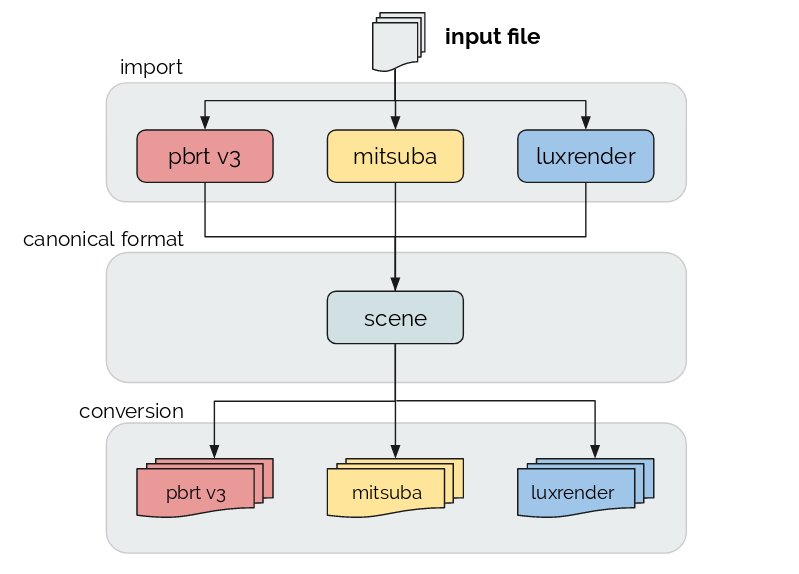
\includegraphics[width=0.8\linewidth]{figs/3_system_architecture/architecture.png}
\caption{Our scene conversion pipeline. An input scene description is converted to a canonical representation, which, in turn, can be exported to a target rendering system format.}
\label{fig:sysarch}
\end{figure}

\subsection{The Import Module}
Most physically-based renderers subdivide the scene description in two main sections:
%Usually, it is divided into two sections: 
{\it scene-wide rendering options} and {\it world block}. The former defines the rendering settings, while the latter describes the scene geometry and materials.
%
The import module parses the input scene files and translates each directive into a canonical
representation. Since rendering systems use proprietary file format, both the import and export modules have to be specialized for each renderer.

PBRT and LuxRender scene descriptions consist of structured text statements \red{(see XXX)}. We generated parsers for these systems using 
%Given their structure, a Lex/Yacc parser was considered the best choice for these formats. As we intended to keep our system in pure Python, we chose to use The parser for  
PLY \cite{ply}, a Python implementation of Lex and Yacc.
%
Mitsuba, in turn, is a heavily optimized, plugin-oriented renderer. Its file
format is, essentialy, a XML description of which plugins should be instantiated
with the specified parameters. Since there are several XML-parsing libraries for Python that can load the hierarchy into a tree data
structure, we chose to use ElementTree \cite{ET}, a Python XML parsing tool.

\subsection{Canonical Scene Representation}
%After loading the scene file, the information has to be stored somewhere. 
While most renderers have a similar structure, they differ in a few supported features and in the parameters used to configure the rendering process. Thus, we need a canonical representation that covers the features supported by all renderers, 
%
 COLLADA~\cite{collada} is an XML schema intended as a representation for exchanging digital content among graphics applications. 
 %Ever since it became property of the 
 %Khronos Group, several companies included a COLLADA module on their 3D modeling 
 %softwares or game engines. However, there were few physically-based renderers 
 %that adhered to this file format, one of the few being Mitsuba. That might have 
 %happened because 
 However, COLLADA files only include information about scene geometry. No information about other rendering 
 options, such as camera positioning or integration techniques, is available. 
 In order to establish a common ground for conversion, we defined a canonical representation for these scenes. Such a representation 
 is illustrated in Figure~\ref{fig:canonicalrep} and can easily extended to incorporate any directives not covered in our current implementation.
 
%Renderer directives are usually written as a command, followed by a type and a list of additional parameters. 
%So, for instance, to specify the path
%integration technique with 8192 samples per pixel in PBRT v3 one would
%write:  
%\texttt{\small Integrator "path" "integer pixelsamples" [8192]}

%In order to establish a common ground for conversion, we decided it best to define a canonical representation for these scenes. This representation can be easily extended to incorporate any directives not contemplated in this work.

Our canonical scene representation mirrors the general structure of scene files and divides the scene data into
scene-wide {\it rendering options} and {\it world block}. 
%The rendering options are subdivided into {\it integration} technique and {\it sensor} options, while the world block is subdivided into  {\it material} definitions, global {\it emitters}, and lists of {\it shapes}. 
This structure is illustrated in Figure~\ref{fig:canonicalrep}, where the attributes stored for each scene component are shown on the rectangles on the right.

\begin{figure}[h]
\centering
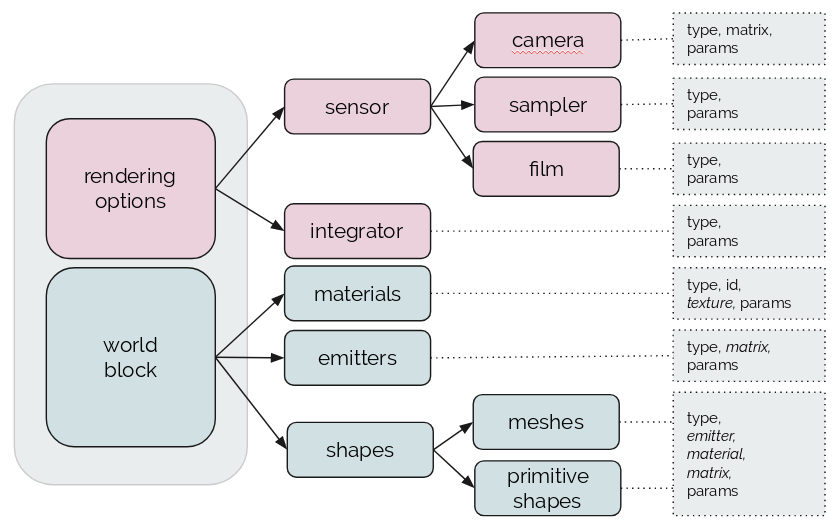
\includegraphics[width=0.9\linewidth]{figs/3_system_architecture/canonicalrep.png}
\caption{Canonical scene representation. It separates rendering options from scene block data. The attributes stored for each component are shown on the rectangles on the right.}
\label{fig:canonicalrep}
\end{figure}

%\subsubsection{Scene-wide Rendering Options}
\noindent \textit{Rendering Options}:
%\noindent \textbf{Rendering Options}
a set of directives specifying the integration and sampling techniques used for
rendering, as well as camera and film properties. These include, for instance, camera position, camera matrix, image resolution, field of view, etc.
%These directives are represented in a structure with two fields: 
\red{[What else?]}.

%\subsubsection{World Block}
\noindent \textit{World Block}:
a set of directives describing the materials, global emitters, and shapes present in the scene.
%
A {\it material} (\eg, glass, metal, plastic, etc.) may have one or more associated textures. {\it Global emitters} represent all kinds of light sources, except area light sources, which are represented as shapes. These include conventional environment, spot, directional, and point light sources, as well more specific ones such as {\it sun} and {\it sky}.
%The \textbf{material} directive is represented in a structure with: a type \red{(examples of types?)}, an id, an optional texture and a list of parameters.
%
A {\it shape} can be a polygonal mesh or a geometric primitive such as a rectangle, disk, cube, or sphere, for instance. 
%an optional area emitter, an optional material reference, an optional transformation matrix and a list of parameters.

%The \textbf{texture} directive is represented in a structure with: a type, an id and a list of parameters. \red{[Where are the textures themselves stored?]}

%The \textbf{global emitter} directive is represented in a structure with: a type, an optional transformation matrix and a list of parameters.

\subsection{The Export Module}

The export module is at the core of our system. While the import module deals with a single proprietary scene representation at a time, the export module has to map between materials and scene properties from two proprietary representations. 
In this case, there are several delicate cases to
consider. Matrix transformations, native shapes, environment mapping coordinates and, mostly, materials are
some of the components that vary greatly between renderers. 
In several situations, there is no direct mapping between them. Still, our system should provide an output representation that, once rendered with the target system, best approximates the results obtained by the source rendering system with the input scene description. 
Achieving such results required extensive experimentation with parameters of the various systems. Next, we discuss a few relevant aspects one should consider.    
  
%After the data is loaded into our canonical representation, it can be converted into any of the supported formats.
% \subsubsection{Converting Matrices}
%\noindent 
\textbf{Matrix Conversion}: 
There are several issues to consider when converting matrices between renderers.
%A few things we had to keep in mind were: 
Do the two renderers use different coordinate systems (either left-handed or right-handed)? 
%does this renderer use a left or right coordinate system? Does this renderer 
Do they represent matrices in the scene file using a direct representation or its
inverse-transpose? How is the object-world transformation represented for
shapes?

Mitsuba uses a right-hand coordinate system, while PBRT and LuxRender use a
left-hand one. This means that, when converting between Mitsuba and the other
two, one has to mirror the x-axis of all camera matrix transformations. This is
also the case for environment map positioning and object-world
transformations. Moreover, Mitsuba's scene files contain a world-to-camera transformation matrix (\ie, view matrix),
while PBRT and LuxRender scene files use the view matrix inverse transpose.

%\green{Furthermore, Mitsuba scene files have their camera position specified as a 
%world-to-camera transformation matrix, while PBRT and LuxRender scene files have 
%theirs as a camera-to-world transformation matrix. Therefore, converting the 
%camera positioning between Mitsuba and the other two renderers means we have to 
%compute the inverse transpose of this transformation matrix.}

% \red{Mitsuba also has its camera transformation matrix specified as a camera-to-world
%  transformation, while PBRT and LuxRender do not. Therefore, when converting the
% camera look-at matrix between these renderers, we had to compute the inverse
% transpose of the specified matrix. }

% \subsubsection{Converting Materials}
\textbf{Material Conversion}: 
materials are the most delicate aspect of scene conversion. Materials have
spectral and roughness properties that absolutely must be correctly mapped. 
However, most renderers have very different implementations
for common subsurface scattering models (BSDFs), making it hard to
predict the mapping between the parameters of two such implementations.

Mitsuba uses a more physics-oriented approach: a material can be diffuse,
conductor, dielectric, plastic, translucent, or a bumpmap.
It also has other types of materials, but those are not supported in the current implementation of our system.
The material type in Mitsuba changes as the material contains any form of
surface roughness, becoming a ``rough'' version of itself (for instance, a rough
metal becomes a roughconductor).
%
PBRT and LuxRender materials have roughness parameters, making it unnecessary to
change the material's name.

%The major problem was faced when converting metals from and to LuxRender. 
To represent the material's reflectance, PBRT and Mitsuba use one index of refraction ($\eta$) and one absorption 
coefficient (\textit{k}) per color channel. 
LuxRender, however, uses a so-called ``{\it Fresnel texture}'', specifying a 
single value of $\eta$ and \textit{k} for all channels. Alternatively, LuxRender allows the specification of a single RGB 
color value for the material's reflectance. Therefore, correctly converting metal colors between LuxRender and PBRT or Mitsuba is not well defined, 
and is not supported in the current implementation of our system.

\textbf{Shape Conversion}: 
shape directives can be split into two categories: {\it primitive shapes}, which can
be used to specify primitives such as {\it rectangles, disks, cubes}, and {\it spheres};
and {\it 3D meshes}, which are stored in external files. 
%
Converting primitive shapes requires more attention than converting external 3D meshes. 
Mitsuba has directives for rectangle, disk, cube and sphere, while PBRT and LuxRender do not. 
Mitsuba's primitives are defined by some parameters (\eg, vertex positions, radius) which can be modified by 
a transformation (model) matrix. To reproduce these primitives in PBRT and 
LuxRender, an {\it internal triangle mesh} must be used. This is done by specifying the position, normal, and texture coordinates for each vertex in the mesh representing a given primitive. One should note that such internal meshes do not use the same representation as the 3D meshes stored in files.

Converting PBRT and LuxRender internal triangle meshes into Mitsuba primitive shapes is a more involving process. Since Mitsuba's 
primitives have predefined coordinates, converting vertices from PBRT or LuxRender internal meshes into 
these coordinates requires obtaining the transformation matrix that maps PBRT or LuxRender vertices 
to Mitsuba's predefined points. Our system takes care of this automatically.

Converting external 3D meshes is simple, as all rendering systems have directives
for this purpose. PBRT, however, does not support Object File Wavefront 3D
(.obj) files. 
%the user with mesh converting tools.
In this case, our system issues a warning, making the user aware of the need to convert .obj files off-line.

% Since the triangle mesh directive specifies each points in world coordinates, 
% The reverse process, however, is more complicated. The triangle mesh directive
% specifies the coordinates, normal and uv mapping for the points forming a
% triangle. In order to recover a transformation matrix for the corresponding
% Mitsuba primitive, \red{these points have to be multiplied by the original Mitsuba
% canonical coordinates in the correct order.}

\textbf{Global Emitter Conversion}:
global emitters can used to emulate environment lighting, such as the sun, the
sky, or an environment map. Converting global emitters can be tricky, mainly
because different rendering systems do not implement the same algorithms and directives. 
For instance, Mitsuba and LuxRender implement {\it sun} and {\it sky} directives, while PBRT does not.
%However, these directives can be converted from Mitsuba and LuxRender to PBRT. 
A sun directive can be simulated in PBRT using a distant light. A sky directive can
be simulated using an environment map of a clear sky.
While PBRT and LuxRender access environment maps using spherical coordinates, 
Mitsuba uses a latitude-longitude format. Thus, a conversion between the two representations is required. 
  
%
Converting a PBRT distant light into
a sun directive for Mitsuba or LuxRender is straightforward. However, converting a PBRT
environment map into a sky directive lends to an ambiguous situation, as the converter would require additional information to decide 
whether the environment map should be treated just as a regular environment map, or as a sky directive.
Our system solves this ambiguity by asking the user if the environment map should be converted to a sky
emitter.

%%Another sensitive point to consider is converting environment mapping indexation. 
%PBRT and LuxRender access environment maps using spherical coordinates, 
%%($\theta$, $\phi$), 
%while Mitsuba uses a latitude-longitude format.   
%%(\textit{x}, \textit{y} and \textit{z}).
%%, as  shown in Figure \ref{fig:mitdocemitter}. 
%A conversion between the two representations is required. 
%%can be done by applying a \red{transformation matrix on the 
%%environment map, rotating the \textit{x}, \textit{y} and \textit{z} axes to match the differing axis setup.} 

%\begin{figure}[h]
%\centering
%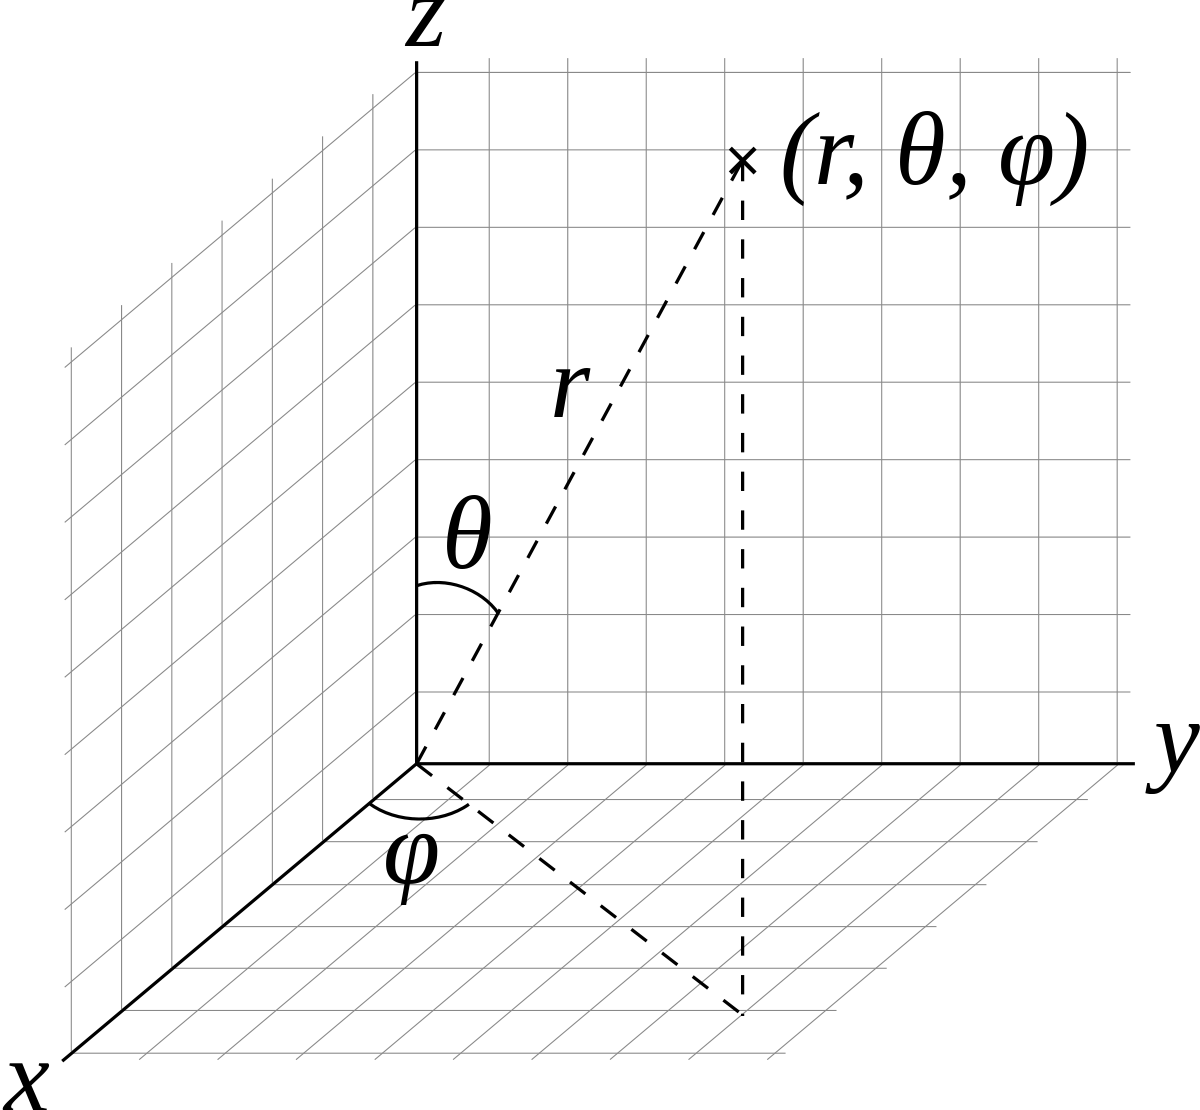
\includegraphics[width=1.2in]{figs/3_system_architecture/spherical_coordinates.png}
%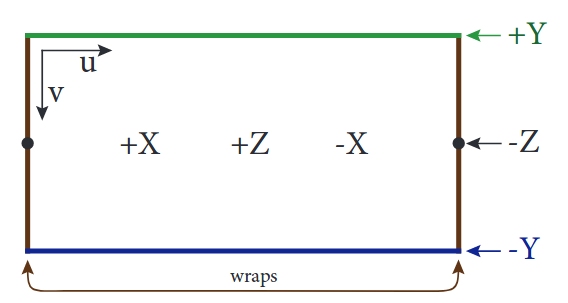
\includegraphics[width=2.0in]{figs/3_system_architecture/mitdocemitter.png}
%\caption{Illustration of the coordinate conventions used by PBRT and LuxRender 
%(left) and by Mitsuba (right) for indexing environment map uv coordinates.}
%\label{fig:mitdocemitter}
%\end{figure}


